\chapter{Introduction}
\label{chap: Introduction}


\section{Background and Motivation}
Turbulent flows are seen in all sorts of natural and engineering systems, from large-scale atmospheric flows and ocean currents to industrial processes and aerodynamic applications. Capturing these turbulent multi-scale flow dynamics has proven to be a formidable challenge, both analytically, numerically, and experimentally. To ensure qualitative research and engineering solutions, an accurate representation of these turbulent dynamics is crucial, yet achieving this with a manageable computational cost has proven to be a challenging problem. 

Over the past decades, Computational Fluid Dynamics (CFD) has proven itself as an effective and powerful way to simulate fluid flow, both laminar and turbulent. It has proven its use across various industries, where it has played a central role in the analysis, design, and certification of aerospace vehicles, environmental systems, industrial products, and even healthcare developments. Advances in numerical methods and high-performance computing (HPC) have ensured steady advances in reliability and accuracy of CFD, making it a critical element in modern engineering workflows \cite{Spalart2016}. 

\subsection{Need for high-fidelity yet efficient simulation}

\begin{wrapfigure}{r}{0.5\textwidth}
\vspace{-1.5em}
     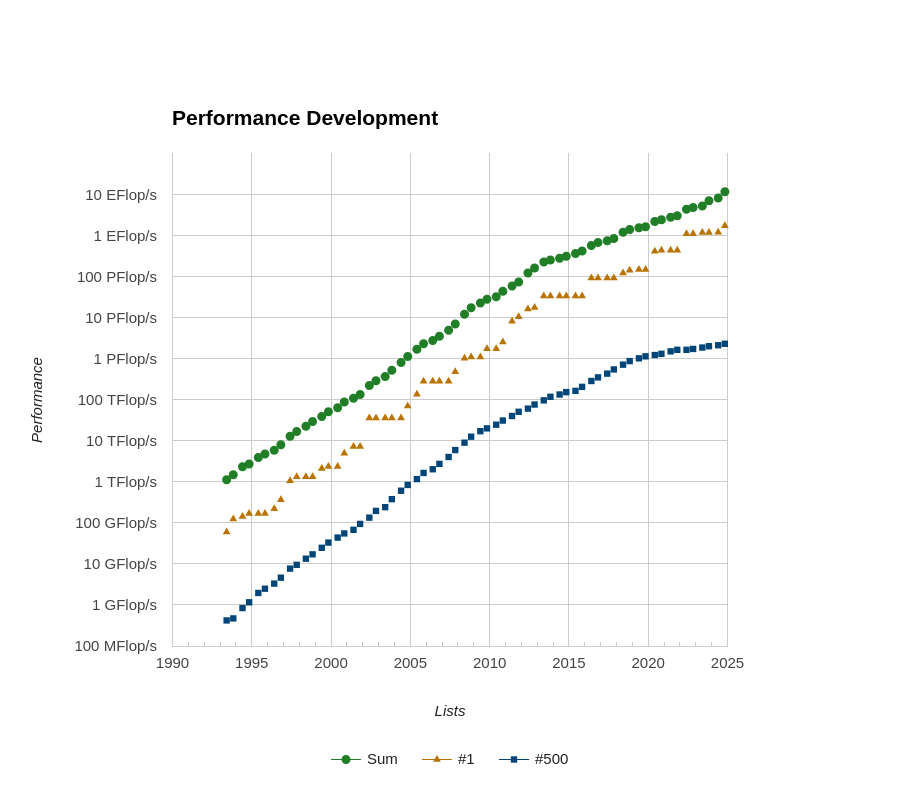
\includegraphics[width=\linewidth]{figures/Moore.png}
    \caption{Performance trends of the TOP500 supercomputers (1993–2025), showing total performance (Sum), top system ($\#$1), and 500th system ($\#$500). Performance is in FLOP/s on a logarithmic scale. Adapted from \textcite{top500}}
    \label{fig: Moore}
\end{wrapfigure}

Even with the technological advancements of the last decades, the computational cost of accurate CFD simulations remains a bottleneck. This is especially the case if one aims to resolve unsteady, turbulent flows in or around complex geometries. These types of simulations require a mesh of such high quality that even the smallest and most complex flow phenomena can be captured accurately \cite{Spalart2000}. This presents two problems, each of which requires a substantial amount of time to evaluate: one is fabricating the mesh through which we want to apply our CFD algorithms, and the other is considering the CFD algorithms and subsequent turbulence models. In practice, companies navigate a spectrum of methods that trade computational efficiency for accuracy, ranging from Reynolds Averaged Navier–Stokes (RANS) to Large-Eddy Simulation (LES), hybrid RANS–LES approaches, and ultimately Direct Numerical Simulation (DNS) to gain a competitive edge in the highly competitive aeronautical markets \cite{Spalart2000}. This indicates the need for frameworks that can decrease the computational costs of high-fidelity CFD simulations. 

Compounding this is the slowing of hardware-driven performance gains. Ever since 1965, following Gordon Moore's stipulation \cite{moore1965}, the number of transistors in a single integrated circuit has doubled approximately every two years, while maintaining a fixed cost, power, and area. However, as transistors reach the atomic scale and fabrication costs continue to rise, the classical technological driver underpinning Moore's Law for 50 years is failing and is anticipated to have flattened by 2025 \cite{Shalf2020}, as shown in \autoref{fig: Moore}. This 'death march' of Moore's Law \cite{Markov2014} opens the door for new hard- and software architectures, as well as creative CFD workflows. 

Besides the recent flattening of Moore's Law, researchers have been passionately innovating for several decades and finding novel ways to reduce the computational cost of CFD simulations. One way accelerated CFD simulations can be achieved is to employ advances in computer multicore architecture that have been brought to us over the last few decades \cite{Hosain2015}. These novel methods enable the use of multicore and manycore CPU (Central Processing Unit) architectures \cite{Hadade2016}, as well as the use of GPU (Graphical Processing Units) to accelerate CFD solvers \cite{Xiang2017}. To achieve desirable acceleration results, these hardware methods have been paired with advanced numerical schemes which employ mesh, mesh-free, or hybrid methods to attain desirable simulation speed-ups \cite{Hosain2015}. 

Together with advances in computing architecture, the rapid progress of Machine Learning (ML) and Artificial Intelligence (AI) offer interesting new strategies for accelerating CFD simulations. Fluid mechanics has always been a field where an enormous amount of data needs to be dealt with. This can be derived from either experimental results or large-scale numerical simulations \cite{Brunton2020}. Together with these vast amounts of data and an increase in the ability to handle this data, ML offers a promising outlook in aiding the acceleration of modern turbulent CFD simulations.

It is in this landscape that the subject of this thesis finds itself. Bounded by the computational bottleneck created by accurate CFD simulations, and driven by technological advancements in AI technology. This thesis aims to deliver a new way of lowering the computational costs of turbulent flow simulations by employing modern AI frameworks. More specifically, this work will focus on using Neural ordinary differential equations to accelerate the time integration step. Since this is, more often than not, the most costly part in mesh based solving algorithms. In light of this context, this thesis aims to answer the following central research question and subquestions:


\begin{center}
\begin{minipage}{0.9\textwidth}
\begin{tcolorbox}[colback=gray!5,colframe=black!80,title=Research Question]
\textbf{How effectively can neural ordinary differential equations accelerate the time integration step in CFD solvers for turbulent flow simulations without compromising accuracy?}

\begin{enumerate}
  \item What are the key bottlenecks in conventional time integration schemes used in turbulent CFD simulations?
  
  \item To what extent can case-specific neural ODEs maintain physical accuracy across different turbulent flow regimes, Reynolds numbers, boundary conditions, and geometric configurations (e.g., symmetric, asymmetric, irregular shapes)?
  
  \item How sensitive is the solution accuracy of neural ODEs to network architecture and training data quality? 
  
  \item How can residuals or loss functions be used to constrain or monitor neural ODE integration quality?
  
\end{enumerate}
\end{tcolorbox}
\end{minipage}
\end{center}
